 \chapter{Przegląd SMT Solverów: Z3, Yices, CVC5}
%Rozdział opisuje zastosowanie 

\section{Z3}
Z3 to wydajny SMT solver dostępny bezpłatnie przez Microsoft Research. Z3 jest solverem dla logiki symbolicznej, będącej podstawą wielu narzędzi inżynierii oprogramowania. Solwery SMT polegają na ścisłej integracji wyspecjalizowanych silników walidacyjnych. Każdy silnik jest elementem ogólnej struktury i implementuje wyspecjalizowane algorytmy. Przykładowo, silnik Z3 dla arytmetyki obejmuje Simplex, cięcia i rozumowanie wielomianowe, podczas gdy silnik dla obsługi ciągów znaków i wyrażeń regularnych korzysta z metod symbolicznych pochodnych języków regularnych. Wspólną cechą wielu algorytmów jest sposób, w jaki wykorzystują dwoistość między znajdowaniem rozwiązań spełniających a dowodów odrzucających. Solver ten integruje również silniki do wnioskowań globalnych i lokalnych oraz globalnej propagacji.
Z3 jest używany w szerokim zakresie zastosowań inżynierii oprogramowania, obejmując weryfikację programów, walidację kompilatorów, testowanie, fuzzing przy użyciu dynamicznego wykonywania symbolicznego, rozwój oprogramowania oparty na modelach, weryfikację sieci i optymalizację.
Z3 może być zbudowany przy użyciu Visual Studio, pliku Makefile lib CMake. Zapewnia obsługę wielu języków programowania, w tym .NET, C, C++, Java, OCaml, Web Assembly i Python.

\subsection{Architektura systemu}


	Z3 integruje nowoczesny solver SAT oparty na DPLL, bazowy solwer dla teorii, który obsługuje równości i funkcje nieinterpretowane, specjalistyczne silniki (dla arytmetyki, tablic itp.) oraz maszynę abstrakcyjną E-matching (dla kwantyfikatorów). Z3 jest zaimplementowany w C++. Schematyczny przegląd Z3 pokazano na poniższym rysunku.	
	

	\begin{figure}
		\centering
		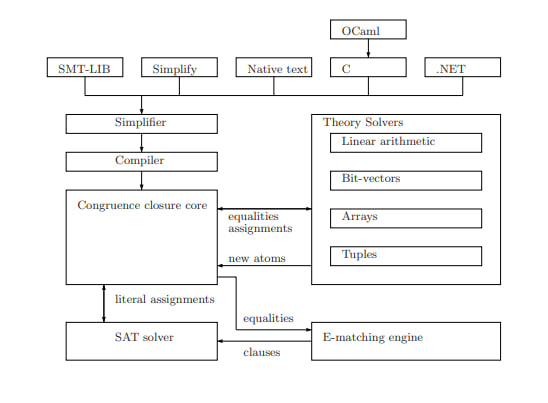
\includegraphics[width=0.7\linewidth]{screenshot001}
		\caption{}
		\label{fig:screenshot001}
	\end{figure}

\textbf{Simplifier}. Formuły wejściowe są najpierw przetwarzane przy użyciu niekompletnego, ale wydajnego uproszczenia. Simplifier stosuje standardowe zasady redukcji algebraicznej, takie jak $p \land true \implies p$, ale także wykonuje ograniczone uproszczenie kontekstowe, identyfikując definicje równościowe w danym kontekście i redukuje pozostałą formułę przy użyciu definicji, na przykład $x = 4 \land q(x) \implies x = 4 \land q(4)$. Trywialnie spełnialny spójnik $x = 4$ nie jest kompilowany do jądra, ale zachowany poza nim na wypadek, gdyby klient wymagał modelu do obliczenia x.

\textbf{Compiler}. Uproszczona abstrakcyjna reprezentacja drzewa składniowego formuły jest przekształcana w inną strukturę danych, składającą się ze zbioru klauzul i węzłów domknięcia kongruencji.

\textbf{Jądro domknięcia kongruencji}. Jądro domknięcia kongruencji otrzymuje przypisania prawdy do atomów od solwera SAT. Atomy obejmują równości i formuły atomowe specyficzne dla danej teorii, takie jak nierówności arytmetyczne. Równości stwierdzone przez SAT solver są przekazywane przez jądro domknięcia kongruencji za pomocą struktury danych, którą nazywamy E-grafem. Węzły w E-grafie mogą wskazywać na jeden lub więcej solverów teorii. Gdy dwa węzły są połączone, zbiór odwołań do teorii są łączone, a samo złączenie jest propagowane jako równość do solverów teorii w przecięciu obu zbiorów odwołan. Jądro również propaguje efekty solverów teorii, takie jak wywnioskowane równości oraz atomy przypisane do wartości true lub false.Solvery teorii mogą także generować nowe atomowe wyrażenia w przypadku teorii niekonweksyjnych. Te atomy są następnie integrowane i zarządzane przez główny solver SAT.

\textbf{Kombinacja teorii}. Tradycyjne metody łączenia solverów teorii opierają się na zdolności tych solwerów do generowania wszystkich wynikających równości lub na wprowadzaniu dodatkowych literałów do przestrzeni poszukiwań na etapie wstępnego przetwarzania. Z3 używa nowej metody kombinacji teorii, która przyrostowo dostosowuje modele utrzymywane przez każdą teorię.

\textbf{SAT Solver}. Podziały przypadków logicznych są kontrolowane za pomocą najnowocześniejszego SAT solwera. Solver SAT integruje standardowe metody przycinania wyszukiwania, takie jak dwa obserwowane literały dla wydajnej propagacji ograniczeń boolowskich, lemma learning z wykorzystaniem klauzul konfliktowych, buforowanie faz w celu kierowania podziałami przypadków i wykonuje niechronologiczny backtracking.

\textbf{Usuwanie klauzul}. Instancjonowanie kwantyfikatorów ma skutek uboczny w postaci tworzenia nowych klauzul zawierających nowe atomy w przestrzeni poszukiwań. Z3 usuwa te klauzule wraz z ich atomami i termami, które były bezużyteczne w zamykaniu gałęzi. Klauzule konfliktowe i zawarte w nich literały nie są natomiast usuwane, dlatego instancje kwantyfikatorów, które były przydatne w wywołaniu konfliktów, są zachowywane jako efekt uboczny.

\textbf{Propagacja relewancji}. Solwery oparte na DPLL(T) przypisują wartość boolowską potencjalnie wszystkim atomom pojawiającym się w wyniku. W praktyce niektóre z tych atomów są nieistotne. Z3 ignoruje te atomy dla kosztownych teorii, jak np. wektory bitowe, i reguł wnioskowania, jak instancjonowanie kwantyfikatorów.

\textbf{Instancjonowanie kwantyfikatorów z użyciem E-matchingu}. Z3 wykorzystuje zaawansowaną technikę do rozumowania kwantyfikatorów, która opiera się na E-grafie. Dzięki nowym algorytmom, które identyfikują dopasowania w E-grafach w sposób skuteczny i przyrostowy, Z3 osiąga znaczną przewagę wydajności w porównaniu do innych nowoczesnych SMT solverów. 

\textbf{Theory Solvers}. Z3 wykorzystuje liniowy solver arytmetyczny oparty na algorytmie używanym w Yices. Teoria tablic stosuje leniwe instancjonowanie aksjomatów tablicowych. Teoria wektorów bitowych o stałym rozmiarze stosuje bitowanie do wszystkich operacji na wektorach bitowych, z wyjątkiem równości.

\textbf{Generowanie modeli}. Z3 pozwala na generowanie modeli jako części danych wyjściowych. Modele przypisują wartości do stałych na wejściu i generują częściowe grafy dla predykatów oraz symboli  funkcji.

\section{Yices}
sdcssdsdf

\section{CVC5}
sdsdcfsdfcdsf